\documentclass[a4paper,12pt]{article}

% Packages
\usepackage[utf8]{inputenc}
\usepackage{geometry}
\usepackage{titlesec}
\usepackage{lipsum} % for generating dummy text
\usepackage{graphicx}
\usepackage{caption}
\usepackage{subcaption}
\usepackage{listings}
\usepackage{amsmath}
\usepackage{amssymb}                                                                                                                                                            
\usepackage{xcolor}

% Page setup
\geometry{a4paper, margin=1in}
\setlength{\parindent}{0pt}
\setlength{\parskip}{5pt}

% Title setup
\title{\textbf{DSP LAB - Experiment 5} \\
        \vspace*{0.3em}
        \large{Design of FIR Filters}}                                                
\author{Ajay Krishnan K \\  EE22BTECH11003}
\date{February 24, 2024}

% Section and subsection formatting
\titleformat{\section}[block]{\normalfont\Large\bfseries}{\thesection}{1em}{}
\titleformat{\subsection}[block]{\normalfont\large\bfseries}{\thesubsection}{1em}{}
\titleformat{\subsubsection}[block]{\normalfont\normalsize\bfseries}{\thesubsubsection}{1em}{}

% Code listing settings
\lstdefinestyle{mystyle}{
    language=Matlab,
    basicstyle=\ttfamily\small,
    breaklines=true,
    keywordstyle=\color{blue},
    commentstyle=\color{green!40!black},
    stringstyle=\color{red},
    % numbers=left,
    % numberstyle=\tiny,
    frame=single,
    showspaces=false,
    showstringspaces=false,
}

\lstset{style=mystyle}

\begin{document}
\maketitle

\section*{Aim}
To design a low-pass and a band-pass FIR filter 
using the windowing method and to verify the design using MATLAB and C.

\section*{Theory}
\subsection*{FIR Filters}
A Finite Impulse Response (FIR) filter is a type of digital filter. 
It is characterized by the fact that its impulse response is of finite 
duration. The impulse response of an LTI system is the output of the 
system when the input is an impulse. The impulse response of an FIR filter
 is always of finite duration because the output of the filter is a 
 weighted sum of the input samples, and the weights are always of finite
  duration.

\subsection*{Windowing Method}
The windowing method is a simple and effective technique for designing
FIR filters. The basic idea is to design an ideal filter and then
truncate and window the impulse response to obtain a practical filter.
The ideal filter is designed by specifying the desired frequency response
and then taking the inverse Fourier transform to obtain the impulse response.
The impulse response is then truncated and windowed to obtain the practical
filter.

\subsection*{Low-pass Filter}
A low-pass filter is a filter that passes signals with a frequency lower
than a certain cutoff frequency and attenuates signals with frequencies
higher than the cutoff frequency. The ideal low-pass filter has a frequency
response that is unity for frequencies less than the cutoff frequency and
zero for frequencies greater than the cutoff frequency.

\subsection*{Band-pass Filter}
A band-pass filter is a filter that passes signals with a frequency within
a certain range and attenuates signals with frequencies outside the range.
The ideal band-pass filter has a frequency response that is zero for
frequencies less than the lower cutoff frequency, unity for frequencies
between the lower and upper cutoff frequencies, and zero for frequencies
greater than the upper cutoff frequency.

\section*{Experiment}
\subsection*{Low-pass Filter}
\subsubsection*{Design}
The design of a low-pass filter involves the following steps:
\begin{enumerate}
    \item Specify the filter order $N$ and the cutoff frequency $\omega_c = \frac{2\pi f_c}{f_s}$.
    \item Design the ideal low-pass filter impulse response $h_d[n]$
    using the formula
    \begin{equation*}
        h_{d}[n] = \begin{cases}
            \frac{\sin(\omega_cn)}{\pi n}, & \text{if } n \neq 0 \\
            \frac{\omega_c}{\pi}, & \text{if } n = 0
        \end{cases}, \quad \frac{-(N-1)}{2} \leq n \leq \frac{N-1}{2}
    \end{equation*}
    \item Window the impulse response using a window function $w(n)$ to
    obtain the final impulse response $h(n)$.
\end{enumerate}

\subsubsection*{MATLAB Implementation}
The following MATLAB code designs a low-pass filter
using the windowing method and plots the frequency response of the filters.

\lstinputlisting[language=Matlab]{../code/lowpass.m}

The corresponding frequency response of the filter is shown in Figure \ref{fig:lowpass-freq}.

\begin{figure}[ht]
    \centering
    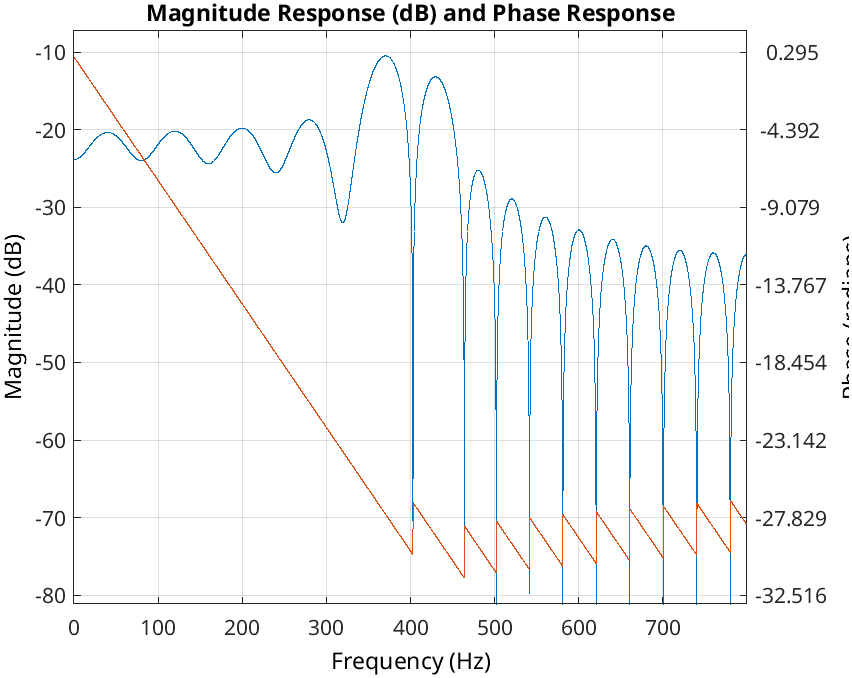
\includegraphics[width=0.8\textwidth]{./figs/LPF_freq.png}
    \caption{Frequency response of low-pass filter designed using MATLAB}
    \label{fig:lowpass-freq}
\end{figure}

\newpage
The corresponding impulse response of the filter is shown in Figure \ref{fig:lowpass-impulse}.
\begin{figure}[ht]
    \centering
    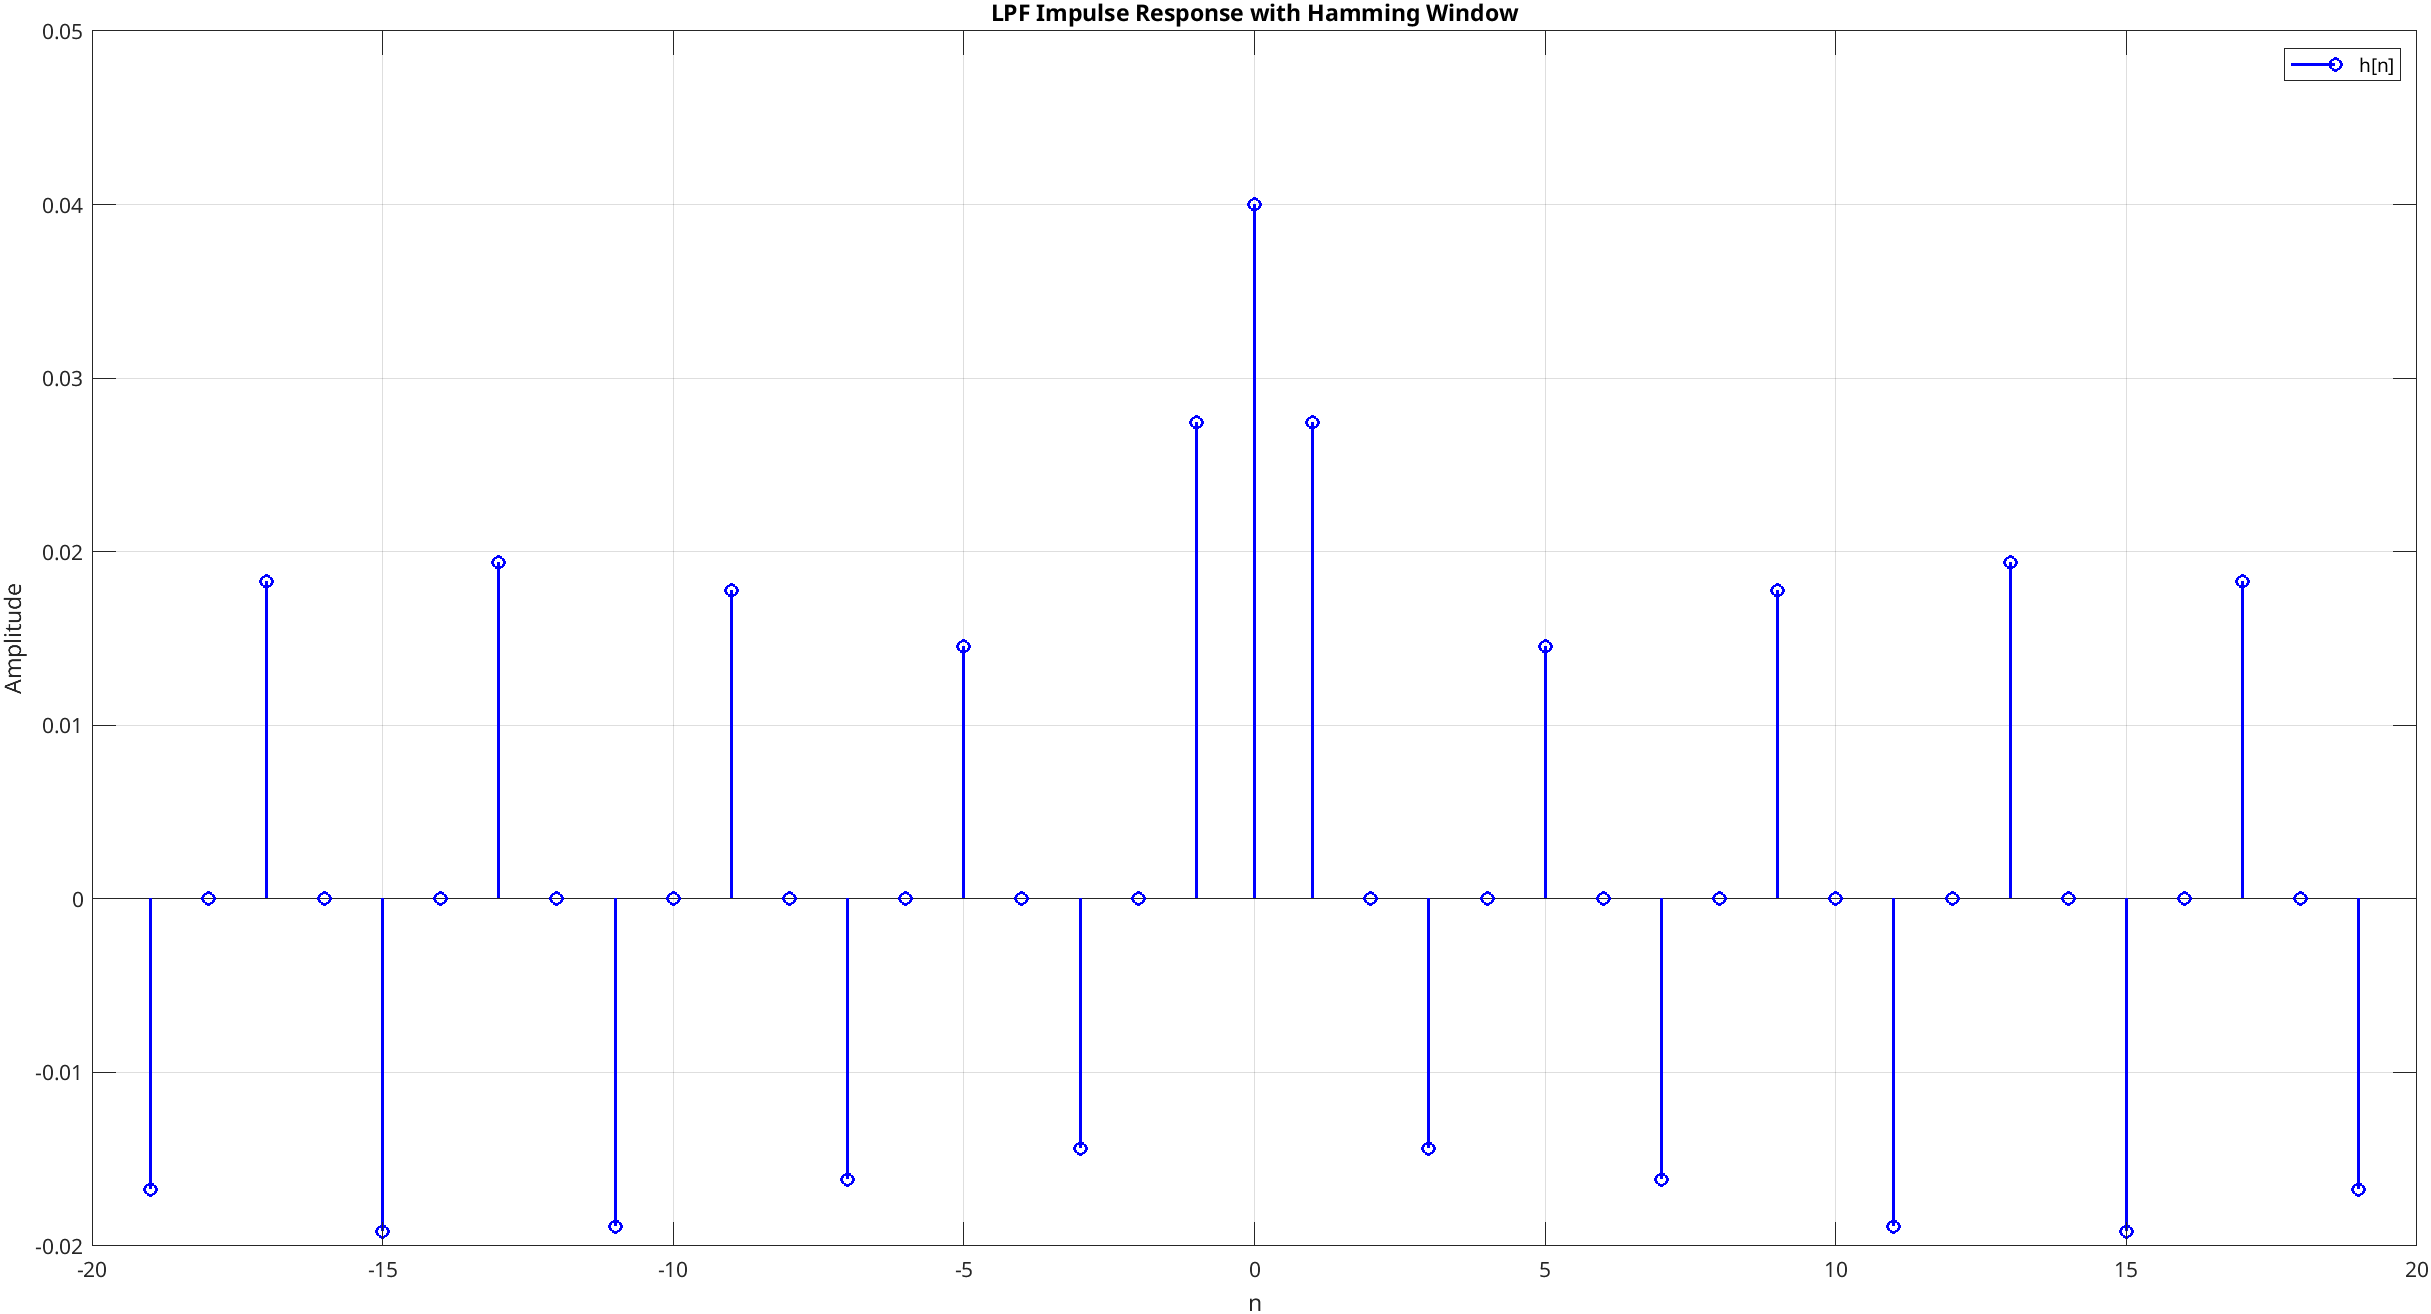
\includegraphics[width=0.8\textwidth]{./figs/LPF_impulse.png}
    \caption{Impulse response of low-pass filter designed using MATLAB}
    \label{fig:lowpass-impulse}
\end{figure}


\subsubsection*{C Implementation}

The following C code designs a low-pass filter using the windowing method.

\lstinputlisting[language=C]{../code/lowpass.c}

The corresponding impulse response of the filter is output as shown :

\begin{lstlisting}
    Impulse Response after Hamming Window:
    0.001333
    0.001451
    0.001460
    0.001096
    0.000000
    -0.002113
    -0.005248
    -0.008961
    -0.012291
    -0.013839
    -0.012016
    -0.005401
    0.006852
    0.024684
    0.046948
    0.071465
    0.095316
    0.115327
    0.128656
    0.133333
    0.128656
    0.115327
    0.095316
    0.071465
    0.046948
    0.024684
    0.006852
    -0.005401
    -0.012016
    -0.013839
    -0.012291
    -0.008961
    -0.005248
    -0.002113
    0.000000
    0.001096
    0.001460
    0.001451
    0.001333
\end{lstlisting}

\subsection*{Band-pass Filter}

\subsubsection*{Design}
The design of a band-pass filter involves the following steps:
\begin{enumerate}
    \item Specify the filter order $N$ and the lower and upper cutoff
    frequencies $\omega_{c1} = \frac{2\pi f_{c1}}{f_s}$ and
    $\omega_{c2} = \frac{2\pi f_{c2}}{f_s}$.
    \item Design the ideal band-pass filter impulse response $h_d[n]$
    using the formula
    \begin{equation*}
        h_{d}[n] = \begin{cases}
            \frac{\sin(\omega_{c2}n) - \sin(\omega_{c1}n)}{\pi n}, & \text{if } n \neq 0 \\
            \frac{\omega_{c2} - \omega_{c1}}{\pi}, & \text{if } n = 0
        \end{cases}, \quad \frac{-(N-1)}{2} \leq n \leq \frac{N-1}{2}
    \end{equation*}
    \item Window the impulse response using a window function $w(n)$ to
    obtain the final impulse response $h(n)$.
\end{enumerate}

\subsubsection*{MATLAB Implementation}
The following MATLAB code designs a band-pass filter
using the windowing method and plots the frequency response of the filters.

\lstinputlisting[language=Matlab]{../code/bandpass.m}

The corresponding frequency response of the filter is shown in Figure \ref{fig:bandpass-matlab}.
\begin{figure}[ht]
    \centering
    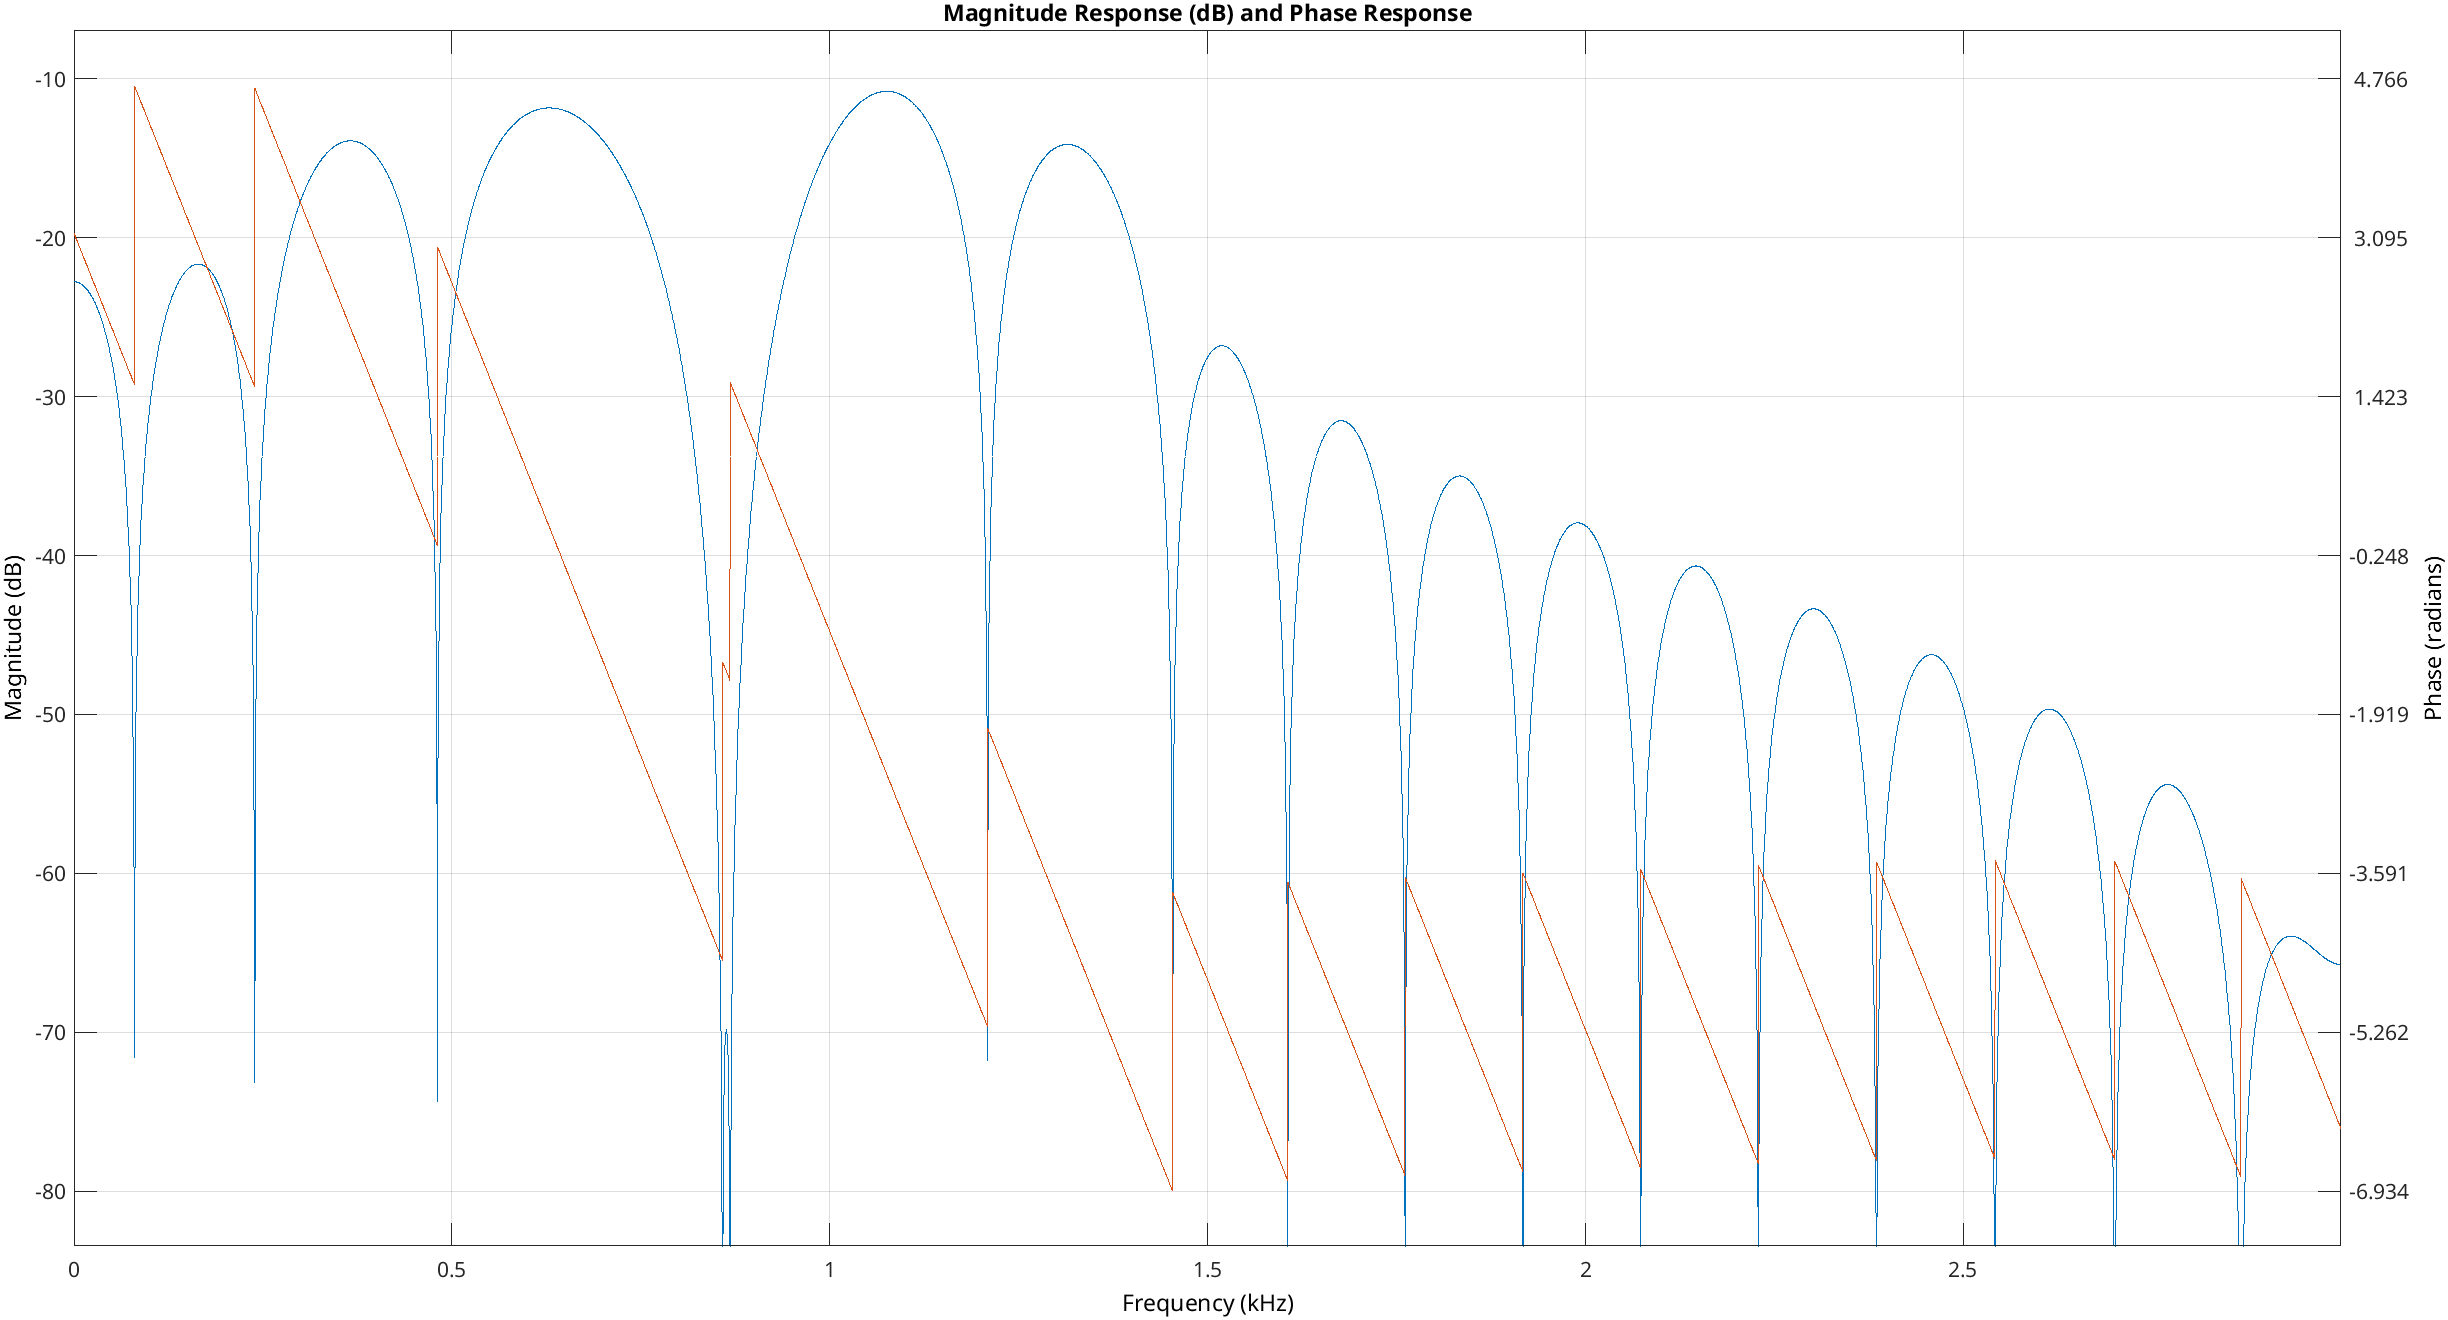
\includegraphics[width=0.8\textwidth]{./figs/BPF_freq.png}
    \caption{Frequency response of band-pass filter designed using MATLAB}
    \label{fig:bandpass-matlab}
\end{figure}

\newpage

The corresponding impulse response of the filter is shown in Figure \ref{fig:bandpass-impulse}.

\begin{figure}[ht]
    \centering
    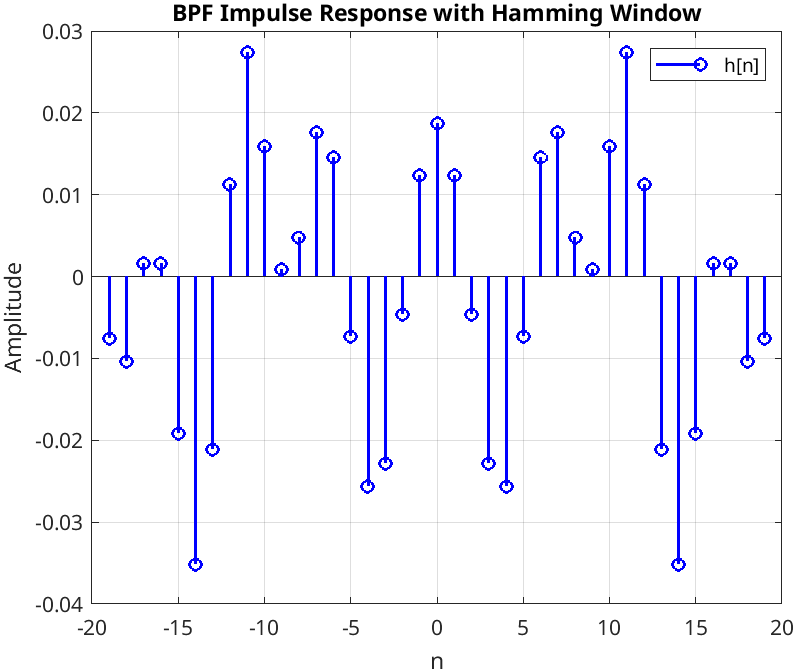
\includegraphics[width=0.8\textwidth]{./figs/BPF_impulse.png}
    \caption{Impulse response of band-pass filter designed using MATLAB}
    \label{fig:bandpass-impulse}
\end{figure}

\subsubsection*{C Implementation}

The following C code designs a band-pass filter using the windowing method.

\lstinputlisting[language=C]{../code/bandpass.c}

The corresponding impulse response of the filter is output as shown :

\begin{lstlisting}
    Impulse Response after Hamming Window:
    -0.000605
    -0.000897
    0.000172
    0.000229
    -0.003756
    -0.009438
    -0.007682
    0.005538
    0.017933
    0.013839
    0.001001
    0.007228
    0.035851
    0.039940
    -0.027106
    -0.130573
    -0.159129
    -0.043180
    0.142675
    0.233333
    0.142675
    -0.043180
    -0.159129
    -0.130573
    -0.027106
    0.039940
    0.035851
    0.007228
    0.001001
    0.013839
    0.017933
    0.005538
    -0.007682
    -0.009438
    -0.003756
    0.000229
    0.000172
    -0.000897
    -0.000605
\end{lstlisting}

\section*{Observations}
\subsection*{Low-pass Filter}
The frequency response of the low-pass filter designed using MATLAB is shown in Figure \ref{fig:lowpass-freq}.
TH cutoff frequency of the filter and the transition band can be observed from the plot.
Based on the given fs and fc, the filter was designed to have higher amount of ripples in the passband and stopband.
This can be reduced by increasing the filter order. By the same way, the transition band can be reduced by increasing the filter order.

The impulse response of the low-pass filter designed using MATLAB is shown in Figure \ref{fig:lowpass-impulse}.
The impulse response of the filter is of finite duration and the windowing method has been used to obtain the practical filter.
The use of windowing method can be observed from the impulse response.

\subsection*{Band-pass Filter}
The frequency response of the band-pass filter designed using MATLAB is shown in Figure \ref{fig:bandpass-matlab}.
The lower and upper cutoff frequencies of the filter and the transition band can be observed from the plot.
Based on the given fs and fc1, fc2, the filter was designed to have higher amount of ripples in the passband and stopband.
This can be reduced by increasing the filter order. By the same way, the transition band can be reduced by increasing the filter order.

The impulse response of the band-pass filter designed using MATLAB is shown in Figure \ref{fig:bandpass-impulse}.
The impulse response of the filter is of finite duration and the windowing method has been used to obtain the practical filter.
The use of windowing method can be observed from the impulse response.

\section*{Conclusion}
The low-pass and band-pass FIR filters
have been designed using the windowing method and the design has been verified using MATLAB and C.
The frequency response and impulse response of the filters have been plotted and the observations have been made.

From the observations, it can be concluded that the windowing method is an effective technique for designing FIR filters.
The stopband and passband ripples can be reduced by increasing the filter order and the transition band can be reduced by increasing the filter order.
Using effective windowing functions can also help in reducing the ripples in the passband and stopband.
Optimising the filter order and the windowing function can help in obtaining the desired frequency response.

\end{document}